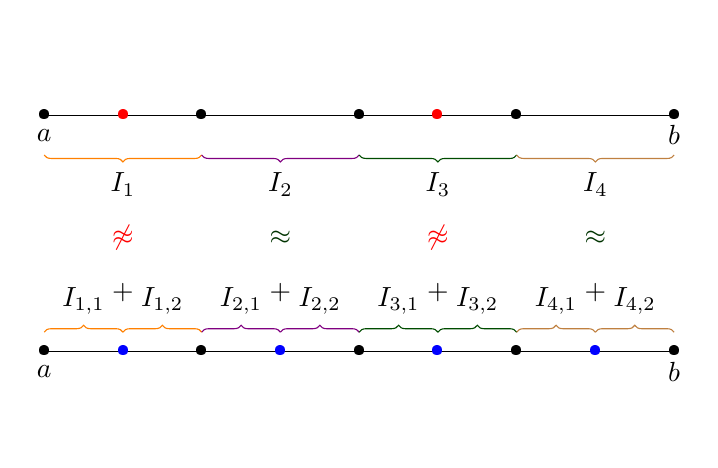
\begin{tikzpicture}
\node at (1,1) {};
\node at (1,-4) {};
% TRAIN
%\draw[<->, dashed] (0,0.5) -- (2,0.5);
%\node at (1,0.75) {$h$};
\draw (0,0) -- (8,0);
\foreach \Point in {(0,0), (2,0), (4,0), (6,0), (8,0)}{\node at \Point {\textbullet};}
\node at (0,-0.25) {$a$};
\node at (8,-0.25) {$b$};

\foreach \Point in {(1,0), (5,0)}{\node[red] at \Point {\textbullet};}

\draw [orange, decorate, decoration = {brace,mirror}] (0,-0.5) -- (2,-0.5)node[pos=0.5,below=3pt,black]{$I_{1}$};

\draw [violet, decorate, decoration = {brace,mirror}] (2,-0.5) -- (4,-0.5)node[pos=0.5,below=3pt,black]{$I_{2}$};

\draw [green!30!black, decorate, decoration = {brace,mirror}] (4,-0.5) -- (6,-0.5)node[pos=0.5,below=3pt,black]{$I_{3}$};

\draw [brown, decorate, decoration = {brace,mirror}] (6,-0.5) -- (8,-0.5)node[pos=0.5,below=3pt,black]{$I_{4}$};

% VALIDATION
%\draw[<->, dashed] (0,-3.5) -- (1,-3.5);
%\node at (0.5,-3.75) {$h/2$};

\draw (0,-3) -- (8,-3);
\foreach \Point in {(0,-3), (2,-3), (4,-3), (6,-3), (8,-3)}{\node at \Point {\textbullet};}
\foreach \Point in {(1,-3), (3,-3), (5,-3), (7,-3)}{\node[blue] at \Point {\textbullet};}
\node at (0,-3.25) {$a$};
\node at (8,-3.25) {$b$};

%\foreach \Point in {(0.5,-3), (1.5,-3), (4.5,-3), (5.5,-3)}{\node[red] at \Point {\textbullet};}

\draw [orange, decorate, decoration = {brace}] (0,-2.75) -- (1,-2.75)node[pos=0.5,above=3pt,black]{$I_{1,1}$};
\draw [orange, decorate, decoration = {brace}] (1,-2.75) -- (2,-2.75)node[pos=0.5,above=3pt,black]{$I_{1,2}$};
\node at (1, -2.25) {$+$};
\node at (1, -1.55) {\textcolor{red}{$\not\approx$}};

\draw [violet, decorate, decoration = {brace}] (2,-2.75) -- (3,-2.75)node[pos=0.5,above=3pt,black]{$I_{2,1}$};
\draw [violet, decorate, decoration = {brace}] (3,-2.75) -- (4,-2.75)node[pos=0.5,above=3pt,black]{$I_{2,2}$};
\node at (3, -2.25) {$+$};
\node at (3, -1.55) {\textcolor{green!20!black}{$\approx$}};

\draw [green!30!black, decorate, decoration = {brace}] (4,-2.75) -- (5,-2.75)node[pos=0.5,above=3pt,black]{$I_{3,1}$};
\draw [green!30!black, decorate, decoration = {brace}] (5,-2.75) -- (6,-2.75)node[pos=0.5,above=3pt,black]{$I_{3,2}$};
\node at (5, -2.25) {$+$};
\node at (5, -1.55) {\textcolor{red}{$\not\approx$}};

\draw [brown, decorate, decoration = {brace}] (6,-2.75) -- (7,-2.75)node[pos=0.5,above=3pt,black]{$I_{4,1}$};
\draw [brown, decorate, decoration = {brace}] (7,-2.75) -- (8,-2.75)node[pos=0.5,above=3pt,black]{$I_{4,2}$};
\node at (7, -2.25) {$+$};
\node at (7, -1.55) {\textcolor{green!20!black}{$\approx$}};
\end{tikzpicture}